\chapter{Visualization of the Linear System of Equations}
\label{appendix-visualization-of-the-linear-system-of-equations}

As shown in the \autoref{chapter-numerical-formulation}, obtaining the pressure distribution in the reservoir for a posterior time step $p^{n+1}$ requires Eq. \ref{equation-single-phase-flow-discretized-linearized} to be solved for each block in the grid.
%
That spans a linear system of $n$ equations in which $n$ is the number of grid blocks in the model.
%
\cite{Ertekin2001} exemplifies this for a tridimensional grid in which $n_x = 4$, $n_y = 3$ and $n_z = 3$, and thus $n = 36$.
%
Figure \ref{figure-parallelepipedal-reservoir-example} shows the reservoir model utilized in this example:
%
\begin{figure}[H]
	\centering
	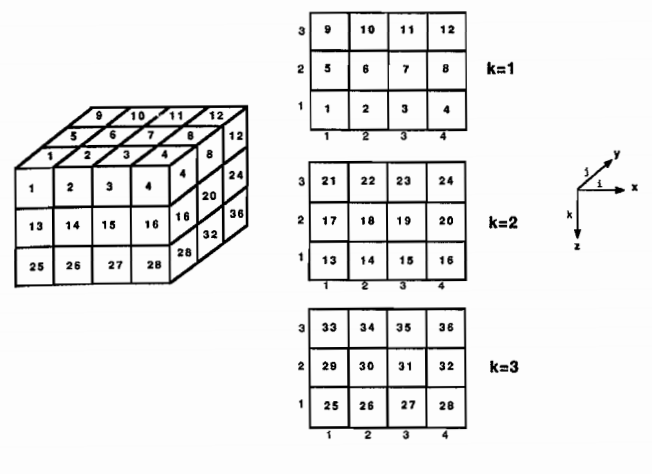
\includegraphics[width=0.8\textwidth]{figure-parallelepipedal-reservoir-example.png}\\
	\caption{Example of a $4 \times 3 \times 3$ grid modeling a parallelepipedal reservoir. Source: \cite{Ertekin2001}.}
	\label{figure-parallelepipedal-reservoir-example}
\end{figure}
\noindent
%
Applying the Eq. \ref{equation-single-phase-flow-discretized-matrix-notation} in the grid block number 1 of this example:
%
\nomenclature[U]{$out$}{Indicates that the grid block is out of the domain of the reservoir}
%
\begin{multline}
	\label{equation-example-evaluation-grid-block-1}
	W^{n+1}_{1}p^{n+1}_{out}+E^{n+1}_{1}p^{n+1}_{2}+S^{n+1}_{1}p^{n+1}_{out}\\+N^{n+1}_{1}p^{n+1}_{5}+B^{n+1}_{1}p^{n+1}_{13}+A^{n+1}_{1}p^{n+1}_{out}+C^{n+1}_{1}p^{n+1}_{1}=Q^{n, n+1}_{1}.
\end{multline}
%
For the sake of simplicity, the indexes $ind$ of Eq. \ref{equation-single-phase-flow-discretized-matrix-notation} were changed to the grid block indexes shown in Figure \ref{figure-parallelepipedal-reservoir-example}.
%
The subscript $out$ indicates that the grid block is out of the domain of the reservoir. 
%
This simulator considers the boundary conditions to be a sealed reservoir, in which there is no flow through the borders of the model. 
%
That can be implemented by assigning a value equals to zero to the transmissibilities of the grid blocks if the transmissibility face is on in a reservoir's boundary. 
%
Thus, Eq. \ref{equation-example-evaluation-grid-block-1} can be simplified as:
%
\begin{multline}
	\label{equation-example-evaluation-grid-block-2}
	E^{n+1}_{1}p^{n+1}_{2}+N^{n+1}_{1}p^{n+1}_{5}+B^{n+1}_{1}p^{n+1}_{13}+C^{n+1}_{1}p^{n+1}_{1}=Q^{n, n+1}_{1}.
\end{multline}
%
For the grid block number 2:
%
\begin{multline}
	\label{equation-example-evaluation-grid-block-3}
	W^{n+1}_{2}p^{n+1}_{1}+E^{n+1}_{2}p^{n+1}_{3}+N^{n+1}_{2}p^{n+1}_{6}+B^{n+1}_{2}p^{n+1}_{14}+C^{n+1}_{2}p^{n+1}_{2}=Q^{n, n+1}_{2}.
\end{multline}
%
For the other grid blocks:
%
\begin{multline}
	W^{n+1}_{3}p^{n+1}_{2}+E^{n+1}_{3}p^{n+1}_{4}+N^{n+1}_{3}p^{n+1}_{7}+B^{n+1}_{3}p^{n+1}_{15}+C^{n+1}_{3}p^{n+1}_{3}=Q^{n, n+1}_{3},
\end{multline}
%
\begin{multline}
	W^{n+1}_{4}p^{n+1}_{3}+N^{n+1}_{4}p^{n+1}_{8}+B^{n+1}_{4}p^{n+1}_{16}+C^{n+1}_{4}p^{n+1}_{4}=Q^{n, n+1}_{4},
\end{multline}
%
\begin{multline}
	E^{n+1}_{5}p^{n+1}_{6}+N^{n+1}_{5}p^{n+1}_{9}+S^{n+1}_{5}p^{n+1}_{1}+B^{n+1}_{5}p^{n+1}_{17}+C^{n+1}_{5}p^{n+1}_{5}=Q^{n, n+1}_{5},
\end{multline}
%
\begin{multline}
	W^{n+1}_{6}p^{n+1}_{5}+E^{n+1}_{6}p^{n+1}_{7}+N^{n+1}_{6}p^{n+1}_{10}+S^{n+1}_{6}p^{n+1}_{2}\\+B^{n+1}_{6}p^{n+1}_{18}+C^{n+1}_{6}p^{n+1}_{6}=Q^{n, n+1}_{6},
\end{multline}
%
\begin{multline}
	W^{n+1}_{7}p^{n+1}_{6}+E^{n+1}_{7}p^{n+1}_{8}+N^{n+1}_{7}p^{n+1}_{11}+S^{n+1}_{7}p^{n+1}_{3}\\+B^{n+1}_{7}p^{n+1}_{19}+C^{n+1}_{7}p^{n+1}_{7}=Q^{n, n+1}_{7},
\end{multline}
%
\begin{multline}
	W^{n+1}_{8}p^{n+1}_{7}+N^{n+1}_{8}p^{n+1}_{12}+S^{n+1}_{8}p^{n+1}_{4}+B^{n+1}_{8}p^{n+1}_{20}+C^{n+1}_{8}p^{n+1}_{8}=Q^{n, n+1}_{8},
\end{multline}
%
\begin{multline}
	E^{n+1}_{9}p^{n+1}_{10}+S^{n+1}_{9}p^{n+1}_{5}+B^{n+1}_{9}p^{n+1}_{21}+C^{n+1}_{9}p^{n+1}_{9}=Q^{n, n+1}_{9},
\end{multline}
%
\begin{multline}
	W^{n+1}_{10}p^{n+1}_{9}+E^{n+1}_{10}p^{n+1}_{11}+S^{n+1}_{10}p^{n+1}_{6}+B^{n+1}_{10}p^{n+1}_{22}+C^{n+1}_{10}p^{n+1}_{10}=Q^{n, n+1}_{10},
\end{multline}
%
\begin{multline}
	W^{n+1}_{11}p^{n+1}_{10}+E^{n+1}_{11}p^{n+1}_{12}+S^{n+1}_{11}p^{n+1}_{7}+B^{n+1}_{11}p^{n+1}_{23}+C^{n+1}_{11}p^{n+1}_{11}=Q^{n, n+1}_{11},
\end{multline}
%
\begin{multline}
	W^{n+1}_{12}p^{n+1}_{11}+S^{n+1}_{12}p^{n+1}_{8}+B^{n+1}_{12}p^{n+1}_{24}+C^{n+1}_{12}p^{n+1}_{12}=Q^{n, n+1}_{12},
\end{multline}
%
\begin{multline}
	E^{n+1}_{13}p^{n+1}_{14}+N^{n+1}_{13}p^{n+1}_{17}+A^{n+1}_{13}p^{n+1}_{1}+B^{n+1}_{13}p^{n+1}_{25}+C^{n+1}_{13}p^{n+1}_{13}=Q^{n, n+1}_{13},
\end{multline}
%
\begin{multline}
	W^{n+1}_{14}p^{n+1}_{13}+E^{n+1}_{14}p^{n+1}_{15}+N^{n+1}_{14}p^{n+1}_{18}+A^{n+1}_{14}p^{n+1}_{2}\\+B^{n+1}_{14}p^{n+1}_{26}+C^{n+1}_{14}p^{n+1}_{14}=Q^{n, n+1}_{14},
\end{multline}
%
\begin{multline}
	W^{n+1}_{15}p^{n+1}_{14}+E^{n+1}_{15}p^{n+1}_{16}+N^{n+1}_{15}p^{n+1}_{19}+A^{n+1}_{15}p^{n+1}_{3}\\+B^{n+1}_{15}p^{n+1}_{27}+C^{n+1}_{15}p^{n+1}_{15}=Q^{n, n+1}_{15},
\end{multline}
%
\begin{multline}
	W^{n+1}_{16}p^{n+1}_{15}+N^{n+1}_{16}p^{n+1}_{20}+A^{n+1}_{16}p^{n+1}_{4}+B^{n+1}_{16}p^{n+1}_{28}+C^{n+1}_{16}p^{n+1}_{16}=Q^{n, n+1}_{16},
\end{multline}
%
\begin{multline}
	E^{n+1}_{17}p^{n+1}_{18}+N^{n+1}_{17}p^{n+1}_{21}+S^{n+1}_{17}p^{n+1}_{13}+A^{n+1}_{17}p^{n+1}_{5}\\+B^{n+1}_{17}p^{n+1}_{29}+C^{n+1}_{17}p^{n+1}_{17}=Q^{n, n+1}_{17},
\end{multline}
%
\begin{multline}
	W^{n+1}_{18}p^{n+1}_{17}+E^{n+1}_{18}p^{n+1}_{19}+N^{n+1}_{18}p^{n+1}_{22}+S^{n+1}_{18}p^{n+1}_{14}\\+A^{n+1}_{18}p^{n+1}_{6}+B^{n+1}_{18}p^{n+1}_{30}+C^{n+1}_{18}p^{n+1}_{18}=Q^{n, n+1}_{18},
\end{multline}
%
\begin{multline}
	W^{n+1}_{19}p^{n+1}_{18}+E^{n+1}_{19}p^{n+1}_{20}+N^{n+1}_{19}p^{n+1}_{23}+S^{n+1}_{19}p^{n+1}_{15}\\+A^{n+1}_{19}p^{n+1}_{7}+B^{n+1}_{19}p^{n+1}_{31}+C^{n+1}_{19}p^{n+1}_{19}=Q^{n, n+1}_{19},
\end{multline}
%
\begin{multline}
	W^{n+1}_{20}p^{n+1}_{19}+N^{n+1}_{20}p^{n+1}_{24}+S^{n+1}_{20}p^{n+1}_{16}+A^{n+1}_{20}p^{n+1}_{8}\\+B^{n+1}_{20}p^{n+1}_{32}+C^{n+1}_{20}p^{n+1}_{20}=Q^{n, n+1}_{20},
\end{multline}
%
\begin{multline}
	E^{n+1}_{21}p^{n+1}_{22}+S^{n+1}_{21}p^{n+1}_{17}+A^{n+1}_{21}p^{n+1}_{9}+B^{n+1}_{21}p^{n+1}_{33}+C^{n+1}_{21}p^{n+1}_{21}=Q^{n, n+1}_{21},
\end{multline}
%
\begin{multline}
	W^{n+1}_{22}p^{n+1}_{21}+E^{n+1}_{22}p^{n+1}_{23}+S^{n+1}_{22}p^{n+1}_{18}+A^{n+1}_{22}p^{n+1}_{10}\\+B^{n+1}_{22}p^{n+1}_{34}+C^{n+1}_{22}p^{n+1}_{22}=Q^{n, n+1}_{22},
\end{multline}
%
\begin{multline}
	W^{n+1}_{23}p^{n+1}_{22}+E^{n+1}_{23}p^{n+1}_{24}+S^{n+1}_{23}p^{n+1}_{19}+A^{n+1}_{23}p^{n+1}_{11}\\+B^{n+1}_{23}p^{n+1}_{35}+C^{n+1}_{23}p^{n+1}_{23}=Q^{n, n+1}_{23},
\end{multline}
%
\begin{multline}
	W^{n+1}_{24}p^{n+1}_{23}+S^{n+1}_{24}p^{n+1}_{20}+A^{n+1}_{24}p^{n+1}_{12}+B^{n+1}_{24}p^{n+1}_{36}+C^{n+1}_{24}p^{n+1}_{24}=Q^{n, n+1}_{24},
\end{multline}
%
\begin{multline}
	E^{n+1}_{25}p^{n+1}_{26}+N^{n+1}_{25}p^{n+1}_{29}+A^{n+1}_{25}p^{n+1}_{13}+C^{n+1}_{25}p^{n+1}_{25}=Q^{n, n+1}_{25},
\end{multline}
%
\begin{multline}
	W^{n+1}_{26}p^{n+1}_{25}+E^{n+1}_{26}p^{n+1}_{27}+N^{n+1}_{26}p^{n+1}_{30}+A^{n+1}_{26}p^{n+1}_{14}+C^{n+1}_{26}p^{n+1}_{26}=Q^{n, n+1}_{26},
\end{multline}
%
\begin{multline}
	W^{n+1}_{27}p^{n+1}_{26}+E^{n+1}_{27}p^{n+1}_{28}+N^{n+1}_{27}p^{n+1}_{31}+A^{n+1}_{27}p^{n+1}_{15}+C^{n+1}_{27}p^{n+1}_{27}=Q^{n, n+1}_{27},
\end{multline}
%
\begin{multline}
	W^{n+1}_{28}p^{n+1}_{27}+N^{n+1}_{28}p^{n+1}_{32}+A^{n+1}_{28}p^{n+1}_{16}+C^{n+1}_{28}p^{n+1}_{28}=Q^{n, n+1}_{28},
\end{multline}
%
\begin{multline}
	E^{n+1}_{29}p^{n+1}_{30}+N^{n+1}_{29}p^{n+1}_{33}+S^{n+1}_{29}p^{n+1}_{25}+A^{n+1}_{29}p^{n+1}_{17}+C^{n+1}_{29}p^{n+1}_{29}=Q^{n, n+1}_{29},
\end{multline}
%
\begin{multline}
	W^{n+1}_{30}p^{n+1}_{29}+E^{n+1}_{30}p^{n+1}_{31}+N^{n+1}_{30}p^{n+1}_{34}+S^{n+1}_{30}p^{n+1}_{26}\\+A^{n+1}_{30}p^{n+1}_{18}+C^{n+1}_{30}p^{n+1}_{30}=Q^{n, n+1}_{30},
\end{multline}
%
\begin{multline}
	W^{n+1}_{31}p^{n+1}_{30}+E^{n+1}_{31}p^{n+1}_{32}+N^{n+1}_{31}p^{n+1}_{35}+S^{n+1}_{31}p^{n+1}_{27}\\+A^{n+1}_{31}p^{n+1}_{19}+C^{n+1}_{31}p^{n+1}_{31}=Q^{n, n+1}_{31},
\end{multline}
%
\begin{multline}
	W^{n+1}_{32}p^{n+1}_{31}+N^{n+1}_{32}p^{n+1}_{36}+S^{n+1}_{32}p^{n+1}_{28}+A^{n+1}_{32}p^{n+1}_{20}+C^{n+1}_{32}p^{n+1}_{32}=Q^{n, n+1}_{32},
\end{multline}
%
\begin{multline}
	E^{n+1}_{33}p^{n+1}_{34}+S^{n+1}_{33}p^{n+1}_{29}+A^{n+1}_{33}p^{n+1}_{21}+C^{n+1}_{33}p^{n+1}_{33}=Q^{n, n+1}_{33},
\end{multline}
%
\begin{multline}
	W^{n+1}_{34}p^{n+1}_{33}+E^{n+1}_{34}p^{n+1}_{35}+S^{n+1}_{34}p^{n+1}_{30}+A^{n+1}_{34}p^{n+1}_{22}+C^{n+1}_{34}p^{n+1}_{34}=Q^{n, n+1}_{34},
\end{multline}
%
\begin{multline}
	W^{n+1}_{35}p^{n+1}_{34}+E^{n+1}_{35}p^{n+1}_{36}+S^{n+1}_{35}p^{n+1}_{31}+A^{n+1}_{35}p^{n+1}_{23}+C^{n+1}_{35}p^{n+1}_{35}=Q^{n, n+1}_{35},
\end{multline}
%
\begin{multline}
	\label{equation-example-evaluation-grid-block-36}
	W^{n+1}_{36}p^{n+1}_{35}+S^{n+1}_{36}p^{n+1}_{32}+A^{n+1}_{36}p^{n+1}_{24}+C^{n+1}_{36}p^{n+1}_{36}=Q^{n, n+1}_{36}.
\end{multline}
%
That constitutes a system of 36 equations with 36 unknowns: the pressures at each of the 36 grid blocks at the next time step $p^{n+1}$.
%
This system can be rewritten as a matrix multiplication in the form:
%
\nomenclature[R]{$A$}{Left-side matrix for the linear system}
\nomenclature[R]{$B$}{Right-side matrix for the linear system}
\nomenclature[R]{$x$}{Pressure matrix for the linear system}
\nomenclature[R]{$n$}{A generic number for representing the number of grid blocks in a matrix}
\nomenclature[U]{$ind$}{Index of the grid block in the example of \autoref{appendix-visualization-of-the-linear-system-of-equations}}
%
\begin{align}
	A x = B.
\end{align}
%
Figure \ref{figure-representation-of-the-linear-system-of-equations} illustrates this system of equations in a matricial form. 
%
The leftmost matrix, $A$, is a sparse matrix, which means it is a matrix composed mostly by zeroes. 
%
Its non-zero members are $A^{n+1}_{ind}$,$N^{n+1}_{ind}$,$E^{n+1}_{ind}$,$C^{n+1}_{ind}$,$W^{n+1}_{ind}$,$S^{n+1}_{ind}$ and $B^{n+1}_{ind}$. $ind$ is equals to the index of the grid block in this example. 
%
For the nature of the problem, each of those coefficients is mapped in a diagonal. 
%
Thus, the coefficient matrix $A$ is a heptadiagonal matrix.
%
\begin{figure}[H]
	\centering
	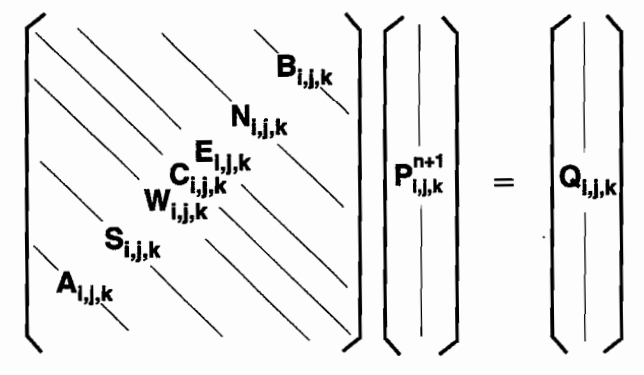
\includegraphics[width=0.7\textwidth]{figure-representation-of-the-linear-system-of-equations.png}\\
	\caption{Representation of the system of equations originated in the simulation of the reservoir described by Figure \ref{figure-parallelepipedal-reservoir-example}. Source: \cite{Ertekin2001}.}
	\label{figure-representation-of-the-linear-system-of-equations}
\end{figure}
\noindent
%
The non-zero entries in the coefficient matrix, the left-side matrix shown in Figure \ref{figure-representation-of-the-linear-system-of-equations}, are shown in the Figure \ref{figure-coefficient-matrix-format} bellow:
%
\begin{figure}[H]
	\centering
	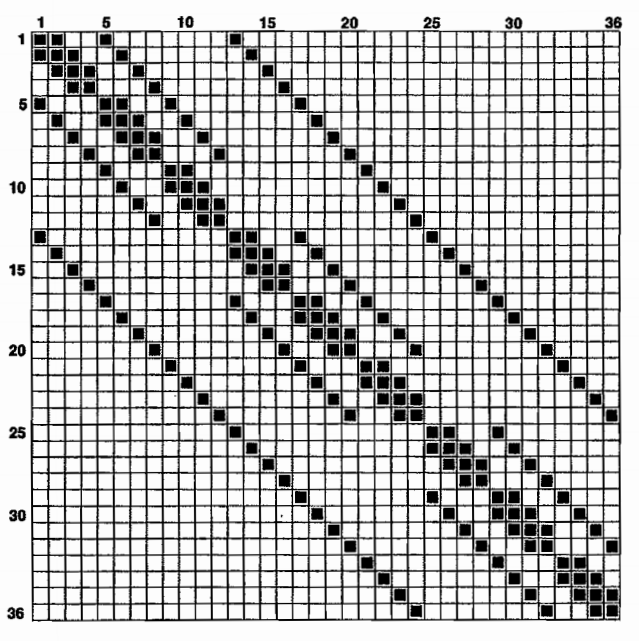
\includegraphics[width=0.7\textwidth]{figure-coefficient-matrix-format.png}\\
	\caption{Coefficient matrix of the system of equations originated from the \cite{Ertekin2001} example of a $ 4 \times 3 \times 3 $  reservoir with sealed boundaries. The black squares represent the non-zero entries. Source: \cite{Ertekin2001}.}
	\label{figure-coefficient-matrix-format}
\end{figure}